\documentclass[11pt]{article}

\usepackage[margin=1in]{geometry}
\usepackage{array}
\usepackage{booktabs}
\usepackage{graphicx}
\usepackage{hyperref}
\usepackage{longtable}
\usepackage{enumitem}
\usepackage[T1]{fontenc}
\usepackage{xurl}

\emergencystretch=3em

\hypersetup{
  colorlinks=true,
  linkcolor=blue,
  urlcolor=blue,
  citecolor=blue
}

\title{Context-Optimized Multi-Agent Orchestration: A Reproducibility Review and Runtime Evaluation}
\author{Context Optimized Agents Project}
\date{May 23, 2026}

\begin{document}

\maketitle

\begin{abstract}
This paper evaluates \texttt{context\_optimized\_agents}, a Python implementation of a scoped-context multi-agent orchestration pattern. The system routes a user objective into role-specific context packets, applies token budgets, audits packets for redundant context, executes 35 specialized agents, compresses findings through parent agents, and records a final decision-memory artifact. We reviewed the implementation, ran its local verification gates, executed the deterministic workflow, generated its metrics and architecture diagram, and tested the OpenAI live integration with \texttt{gpt-5.5}.

The deterministic workflow completed successfully with 35 agent results, 7 parent results, 35 audited packets, no over-budget packets, a quality score of 0.91, and a hallucination-exposure score of 0.18. The included simulator reports a 74.1\% input-token reduction, 56.5\% output-token reduction, 68.6\% estimated token-cost reduction, and 34.3\% latency reduction versus a brute-force broadcast baseline. These metrics remain simulated planning estimates rather than measured production benchmarks. Live OpenAI access was valid, but the full live workflow failed because strict JSON responses were truncated at \texttt{max\_output\_tokens} and parsed without checking \texttt{response.status} or \texttt{incomplete\_details}. This is the primary remaining blocker for production use.
\end{abstract}

\section{Research Questions}

\begin{enumerate}
  \item Does the repository implement the advertised context-optimized orchestration topology?
  \item Does the runnable workflow complete under the declared local test path?
  \item Are the reported metrics measured, simulated, internally consistent, and reproducible?
  \item What remains before the project can be treated as production-grade live OpenAI orchestration?
\end{enumerate}

\section{Methods}

\subsection{Repository and Environment}

The project was evaluated from \texttt{/Users/0xnexis/Desktop/context\_optimized\_agents} on May 23, 2026. The default \texttt{python3} interpreter was Python 3.9.6, below the package requirement of Python \texttt{>=3.10}, so a Python 3.11.14 virtual environment was created with:

\begin{verbatim}
/opt/homebrew/bin/python3.11 -m venv .venv
.venv/bin/python -m pip install -e '.[all,dev]'
\end{verbatim}

\subsection{Documentation and API Check}

Official OpenAI developer documentation was consulted for current Responses API, Structured Outputs, and \texttt{gpt-5.5} behavior. The docs identify \texttt{gpt-5.5} as a current model ID, describe the Responses API as the recommended API for new projects, and document structured outputs through \texttt{text.format} JSON schema configuration.

\subsection{Verification Commands}

The following gates were run:

\begin{verbatim}
.venv/bin/ruff check .
.venv/bin/python -m compileall -q src tests
.venv/bin/python -m unittest discover -s tests
.venv/bin/pytest -q
.venv/bin/python -m context_optimized_agents run --mode mock \
  --objective-file examples/task_objective.txt \
  --output runs/mock_workflow_result.json --print-final
.venv/bin/python -m context_optimized_agents metrics --output runs/metrics.json
.venv/bin/python -m context_optimized_agents diagram --output-dir docs/figures
\end{verbatim}

OpenAI live mode was tested in three stages: a minimal \texttt{gpt-5.5} Responses API smoke test, the default live CLI workflow, and a controlled live workflow with larger output budgets without changing repository code. The API key was supplied only through a silent stdin prompt into \texttt{OPENAI\_API\_KEY}; no secret was written to the repository.

\section{System Description}

The implemented architecture has the following main modules.

\begin{longtable}{p{0.28\linewidth}p{0.64\linewidth}}
\toprule
Module & Observed role \\
\midrule
\texttt{ContextRouter} & Classifies the task and creates 35 role-specific context packets. \\
\texttt{BudgetAllocator} & Assigns fixed input and output token budgets per agent kind. \\
\texttt{ContextAuditor} & Deduplicates repeated retrieved memory and estimates packet-token savings. \\
\texttt{SpecializedAgent} & Calls the configured LLM client for each scoped packet. \\
\texttt{ParentAgent} & Compresses child findings per parent group. \\
\texttt{OrchestrationAgent} & Coordinates routing, audit, child execution, parent compression, final synthesis, metrics, and decision memory. \\
\texttt{OpenAIResponsesClient} & Calls the OpenAI Responses API with strict JSON Schema output. \\
\bottomrule
\end{longtable}

The local workflow uses a deterministic \texttt{MockLLMClient}; live mode uses OpenAI Responses API calls.

\begin{figure}[htbp]
  \centering
  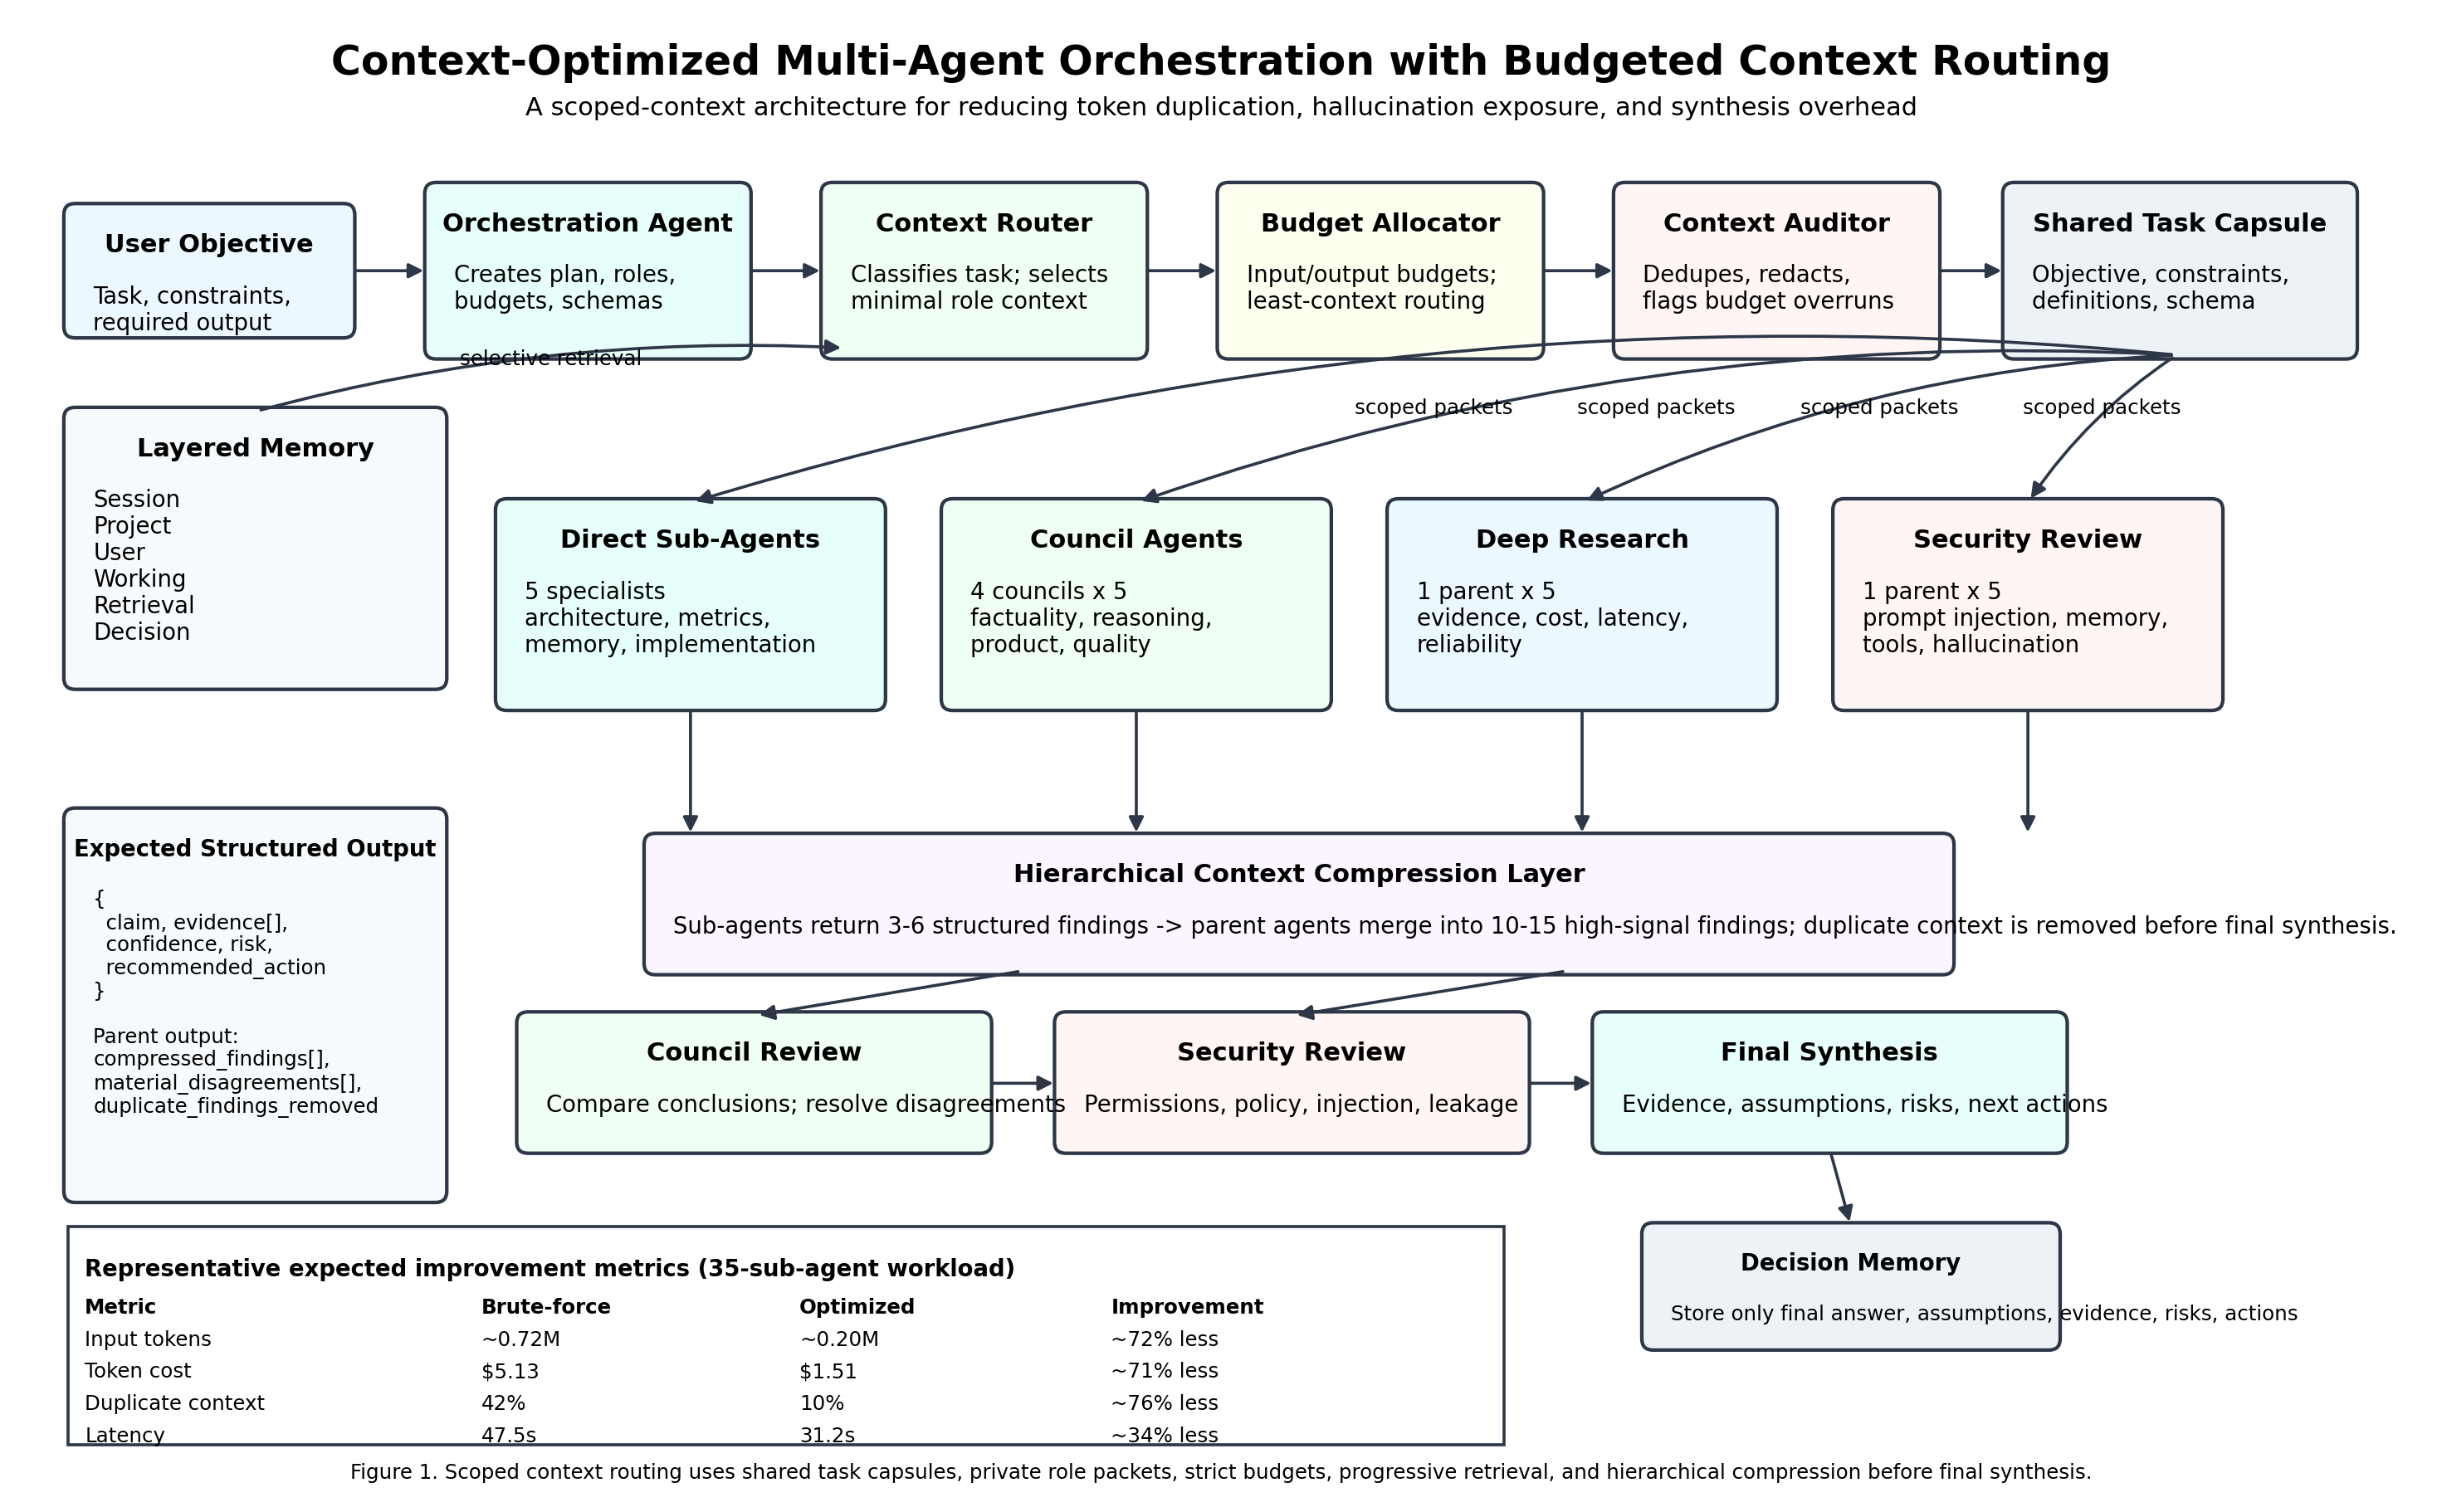
\includegraphics[width=\linewidth]{figures/context_orchestrator_academic_diagram.png}
  \caption{Scoped-context multi-agent orchestration architecture.}
  \label{fig:architecture}
\end{figure}

\section{Results}

\subsection{Local Quality Gates}

\begin{longtable}{p{0.26\linewidth}p{0.14\linewidth}p{0.52\linewidth}}
\toprule
Gate & Result & Evidence \\
\midrule
Python requirement & Pass & Default Python 3.9.6 was unsuitable; \texttt{.venv} used Python 3.11.14. \\
Dependency install & Pass & \texttt{.[all,dev]} installed successfully. \\
Bytecode compilation & Pass & \texttt{compileall -q src tests} exited 0. \\
Unit tests & Pass & \texttt{unittest}: 4 tests passed. \\
Pytest & Pass & \texttt{pytest -q}: 4 tests passed. \\
Ruff lint & Pass after cleanup & 25 fixable \texttt{F401} unused-import violations were removed before repository push. \\
CodeRabbit review & Blocked & CLI authenticated, but the directory was not a git repository during the original review pass. \\
\bottomrule
\end{longtable}

\subsection{Deterministic Workflow Run}

The mock-mode run completed and wrote \texttt{runs/mock\_workflow\_result.json}.

\begin{longtable}{lr}
\toprule
Measurement & Value \\
\midrule
Agent results & 35 \\
Parent results & 7 \\
Audited packets & 35 \\
Estimated input tokens before audit & 30,451 \\
Estimated input tokens after audit & 15,513 \\
Duplicate-context tokens removed & 17,554 \\
Over-budget packets & 0 \\
Audit warnings & 0 \\
Final quality score & 0.91 \\
Hallucination-exposure score & 0.18 \\
\bottomrule
\end{longtable}

The result confirms the deterministic path can execute end-to-end, produce structured findings, perform parent compression, and create a decision-memory record.

\subsection{Simulated Metrics}

The metrics command wrote \texttt{runs/metrics.json}. These values are explicitly simulated for a representative workload, not measured from production traces.

\begin{longtable}{lrrr}
\toprule
Metric & Brute-force & Context-optimized & Improvement \\
\midrule
Input tokens & 701,000 & 181,700 & 74.1\% less \\
Output tokens & 53,600 & 23,300 & 56.5\% less \\
Estimated token cost & \$5.113 & \$1.6075 & 68.6\% less \\
Duplicate-context ratio & 0.42 & 0.10 & 76.2\% less \\
Mean prompt-to-final latency & 47.5 s & 31.2 s & 34.3\% less \\
Hallucination-exposure score & 0.34 & 0.18 & 47.1\% lower \\
Relevant-context density & 0.46 & 0.81 & 76.1\% higher \\
\bottomrule
\end{longtable}

\subsection{OpenAI Live Results}

The \texttt{gpt-5.5} smoke test succeeded and returned the expected output. This confirms network access, credential validity, and model access.

The default live CLI workflow failed before writing \texttt{runs/live\_workflow\_result.json}. The failure occurred while parsing \texttt{response.output\_text} as JSON:

\begin{verbatim}
json.decoder.JSONDecodeError: Unterminated string starting at:
line 1 column 3258
\end{verbatim}

A single-agent probe reproduced the failure and showed the cause.

\begin{longtable}{ll}
\toprule
Field & Value \\
\midrule
Response status & \texttt{incomplete} \\
Incomplete reason & \texttt{max\_output\_tokens} \\
Input tokens & 1,144 \\
Output tokens & 600 \\
Reasoning tokens & 35 \\
Output text length & 3,248 characters \\
Parse result & \texttt{JSONDecodeError} \\
\bottomrule
\end{longtable}

The direct-sub-agent output budget is 600 tokens, while the strict JSON schema can require more than that when the model returns several full findings and issues. The client does not check \texttt{response.status}, \texttt{incomplete\_details}, or refusal content before attempting \texttt{json.loads}. A controlled live run with expanded budgets progressed past the child-agent stage but later failed in parent synthesis with the same truncated JSON pattern at line 1 column 5721.

\section{Findings: What Is Missing and What Remains}

\subsection{Live OpenAI Mode Is Not Production-Ready}

The most important missing piece is robust handling for incomplete structured responses. The live client sends strict JSON schema requests, then parses \texttt{response.output\_text} directly in \texttt{generate\_json}. It should first check \texttt{response.status}, \texttt{incomplete\_details}, refusal content, SDK parse helpers where available, and retryability or budget escalation policy.

\subsection{Topology and Metrics Disagree}

Documentation and metrics describe 6 parent agents, but the actual mock result contains 7 parent groups:

\begin{verbatim}
council_factuality
council_product
council_quality
council_reasoning
deep_research
direct_subagents
security_review
\end{verbatim}

The implementation creates one parent for \texttt{direct\_subagents}, one for \texttt{deep\_research}, one for \texttt{security\_review}, and one for each of four council groups. That is 7 parent agents, not 6. The metrics simulator assumes \texttt{parent\_agents = 6}, and tests only assert \texttt{len(result.parent\_results) >= 6}, which masks the mismatch.

\subsection{Metrics Are Useful but Not Empirical Benchmarks}

The simulator is transparent and reproducible, but it is not a measured benchmark. Claims about latency, duplicate-context ratio, hallucination exposure, relevant-context density, and cost should remain labeled as simulated until a harness measures actual API input/output tokens, cached-token effects, retry and failure rates, wall-clock latency, a brute-force baseline, and measured answer quality.

\subsection{Static Gates and Test Coverage Need Expansion}

The pushed repository now passes Ruff after cleanup, but it still declares \texttt{py.typed} without a configured strict type checker such as mypy or pyright. The current tests confirm deterministic happy paths only. Missing tests include exact parent topology, live-client \texttt{status=incomplete} handling, refusal handling, schema budget sizing, CLI failure modes, retry/backoff behavior, and partial artifact persistence.

\subsection{Failure Isolation and Observability Are Underdeveloped}

The live workflow uses \texttt{asyncio.gather} in a way that fails the whole run on a single agent or parent parse error. Production orchestration should preserve per-agent status, usage, timings, raw response metadata, and recoverable partial outputs. It should also provide progress reporting and structured error summaries.

\section{Discussion}

The project successfully demonstrates the intended local pattern: scoped context packets, role-specific budgets, audit-time deduplication, hierarchical compression, and decision-memory output. The deterministic run proves the control flow is coherent under mocked LLM behavior.

The live runs reveal the boundary between a convincing simulation and a production LLM system. Strict JSON schema output is the right direction, but strict schema does not remove the need to handle incomplete responses, refusals, budget exhaustion, parse failures, retries, and usage telemetry. The current implementation assumes that \texttt{output\_text} is present and parseable. That assumption is false in ordinary live operation when \texttt{max\_output\_tokens} is reached.

The parent-agent count mismatch is also material. A system evaluating context efficiency must align its documented topology, runtime topology, tests, and metrics model. Otherwise, the token and cost results are internally inconsistent even when the simulator is deterministic.

\section{Recommendations}

\begin{enumerate}[leftmargin=*]
  \item Replace direct \texttt{json.loads(response.output\_text)} with a response-normalization layer that handles completed, incomplete, refused, and malformed responses explicitly.
  \item Recalibrate output budgets against each schema using live probes, then add regression tests that fail if schema-conformant outputs no longer fit.
  \item Decide whether the intended topology has 6 or 7 parent agents, then update implementation, docs, metrics, and tests to match.
  \item Add measured benchmark mode that records API usage, latency, success rate, parse retries, and token cost for both brute-force and optimized variants.
  \item Add a strict type checker because the package ships \texttt{py.typed}.
  \item Persist partial live-run artifacts so one failed agent does not erase all completed evidence.
  \item Rotate any API key used for live evaluation if it was shared outside a local secret manager.
\end{enumerate}

\section{Conclusion}

\texttt{context\_optimized\_agents} is a coherent deterministic prototype for scoped-context multi-agent orchestration. Its local run and simulated metrics support the architectural claim that role-specific routing and hierarchical compression can reduce context volume. However, the project is not yet production-grade live orchestration. The remaining work is concentrated in live response handling, budget calibration, topology consistency, empirical benchmarking, type gates, and failure observability.

\section{Reproducibility Artifacts}

Generated artifacts from this evaluation:

\begin{itemize}
  \item \texttt{runs/mock\_workflow\_result.json}
  \item \texttt{runs/metrics.json}
  \item \texttt{docs/figures/context\_orchestrator\_academic\_diagram.svg}
  \item \texttt{docs/figures/context\_orchestrator\_academic\_diagram.png}
  \item \texttt{docs/figures/context\_orchestrator\_academic\_diagram.pdf}
\end{itemize}

\begin{thebibliography}{9}
\bibitem{responses} OpenAI. Responses API Overview. \url{https://developers.openai.com/api/reference/responses/overview}
\bibitem{migration} OpenAI. Migrate to the Responses API. \url{https://developers.openai.com/api/docs/guides/migrate-to-responses}
\bibitem{structured} OpenAI. Structured model outputs. \url{https://developers.openai.com/api/docs/guides/structured-outputs}
\bibitem{gpt55} OpenAI. GPT-5.5 model documentation. \url{https://developers.openai.com/api/docs/models/gpt-5.5}
\bibitem{latest} OpenAI. Using GPT-5.5. \url{https://developers.openai.com/api/docs/guides/latest-model}
\end{thebibliography}

\end{document}
